\documentclass[12pt,a4paper]{article}
\usepackage{cmap} % Makes the PDF copiable. See http://tex.stackexchange.com/a/64198/25761
\usepackage[T1]{fontenc}
\usepackage[brazil]{babel}
\usepackage[utf8]{inputenc}
\usepackage{amsmath}
\usepackage{amsfonts}
\usepackage{amssymb}
\usepackage{amsthm}
\usepackage{textcomp} % \degree
\usepackage{gensymb} % \degree
\usepackage[usenames,svgnames,dvipsnames]{xcolor}
\usepackage{hyperref}
\usepackage{graphicx}
\usepackage[margin=2cm]{geometry}

\hypersetup{
    colorlinks = true,
    allcolors = {blue}
}

% TODO: Consider using exsheets
% http://linorg.usp.br/CTAN/macros/latex/contrib/exsheets/exsheets_en.pdf
%
% http://ctan.org/tex-archive/macros/latex/contrib/exercise/
% Options: answerdelayed,lastexercise,noanswer
\usepackage[answerdelayed,lastexercise]{exercise}

\addto\captionsbrazil{%
\def\listexercisename{Lista de exerc\'icios}%
\def\ExerciseName{Exerc\'icio}%
\def\AnswerName{Solu\c{c}\~ao do exerc\'icio}%
\def\ExerciseListName{Ex.}%
\def\AnswerListName{Solu\c{c}\~ao}%
\def\ExePartName{Parte}%
\def\ArticleOf{de\ }%
}

\renewcommand{\ExerciseHeaderTitle}{(\ExerciseTitle)\ }
\renewcommand{\ExerciseListHeader}{%\ExerciseHeaderDifficulty%
\textbf{%\ExerciseListName\
\ExerciseHeaderNB.\ %
%\ --- \ 
\ExerciseHeaderTitle}%
%\ExerciseHeaderOrigin
\ignorespaces}
\renewcommand{\AnswerListHeader}{\textbf{\ExerciseHeaderNB.\ (\AnswerListName)\ }}

\newcommand{\fixme}{{\color{red}(...)}}

\renewcommand{\theenumi}{\alph{enumi}}
\renewcommand\labelenumi{(\theenumi) }

\newcommand*\tipo{Prova IV}
\newcommand*\turma{PRO112-01U}
\newcommand*\disciplina{GAN0001}
\newcommand*\eu{Helder G. G. de Lima}
\newcommand*\data{06/12/2016}

\author{\eu}
\title{\tipo - \disciplina}
\date{\data}

\begin{document}
\thispagestyle{empty}
\newgeometry{margin=2cm,bottom=0.5cm}
\begin{center}

\includegraphics[width=9.0cm]{marca} \\
\textbf{\tipo\ (\disciplina / \turma)} \\
Prof. \eu\footnote{
Este é um material de acesso livre distribuído sob os termos da licença \href{https://creativecommons.org/licenses/by-sa/4.0/deed.pt_BR}{Creative Commons BY-SA 4.0}.}
\end{center}

\noindent Nome do(a) aluno(a): \underline{\hspace{9,7cm}} Data: \underline{\data}

%\section*{Instruções}
\begin{center}\fbox{
\begin{minipage}{14cm}

{\footnotesize
\begin{itemize}
\renewcommand{\theenumi}{\Roman{enumi}}
\item Identifique-se em todas as folhas.
\item Mantenha o celular e os demais equipamentos eletrônicos desligados durante a prova.
\item Escolha os itens a resolver de modo a totalizar até 10,0 pontos.
\end{itemize}
}

\end{minipage}
}
\end{center}

%\section*{Questões}
\begin{ExerciseList}
\Exercise[title={2,5}] Considere os pontos cujas coordenadas esféricas $\left(r,\theta,\phi \right)$ são $A= \left(12, \frac{\pi}{6}, \frac{\pi}{4}\right)$, $B=(5,\pi,\frac{\pi}{2})$ e $C=(20\sqrt{2},0,\frac{\pi}{4})$. Determine quais destes pontos pertencem ao paraboloide elíptico cuja equação em coordenadas cartesianas é $\frac{y^2}{9} + \frac{z^2}{16} = x+5$.
\Answer \fixme
%$A= (3\sqrt{6},3\sqrt{6},6)$
%$B= (-5,0,0)$

\Exercise[title={2,5}] Identifique e represente graficamente a superfície cuja equação em coordenadas cartesianas é $x^2 + y^2 = 4$. Obtenha equações equivalentes em coordenadas esféricas e cilíndricas.
\Answer \fixme


\Exercise[title={2,5}] Considere o hiperboloide de uma folha ilustrado na \autoref{fig:hip-1}.
\begin{figure}[h]
    \centering
    \begin{minipage}{0.65\textwidth}
    	Sabendo que a interseção desta superfície quádrica com o plano $z=0$ é uma circunferência de raio $2$ e centro $C=(3,0,0)$, e que o ponto $P=(5,-4,-2)$ pertence à superfície, explique como obter (e obtenha) as equações em coordenadas cartesianas, devidamente simplificadas, para:
		\begin{enumerate}
		\item A superfície
		\item A curva formada pela sua interseção com o plano $x=7$.
		\end{enumerate}
    \end{minipage}\hfill
    \begin{minipage}{0.30\textwidth}
        \centering
        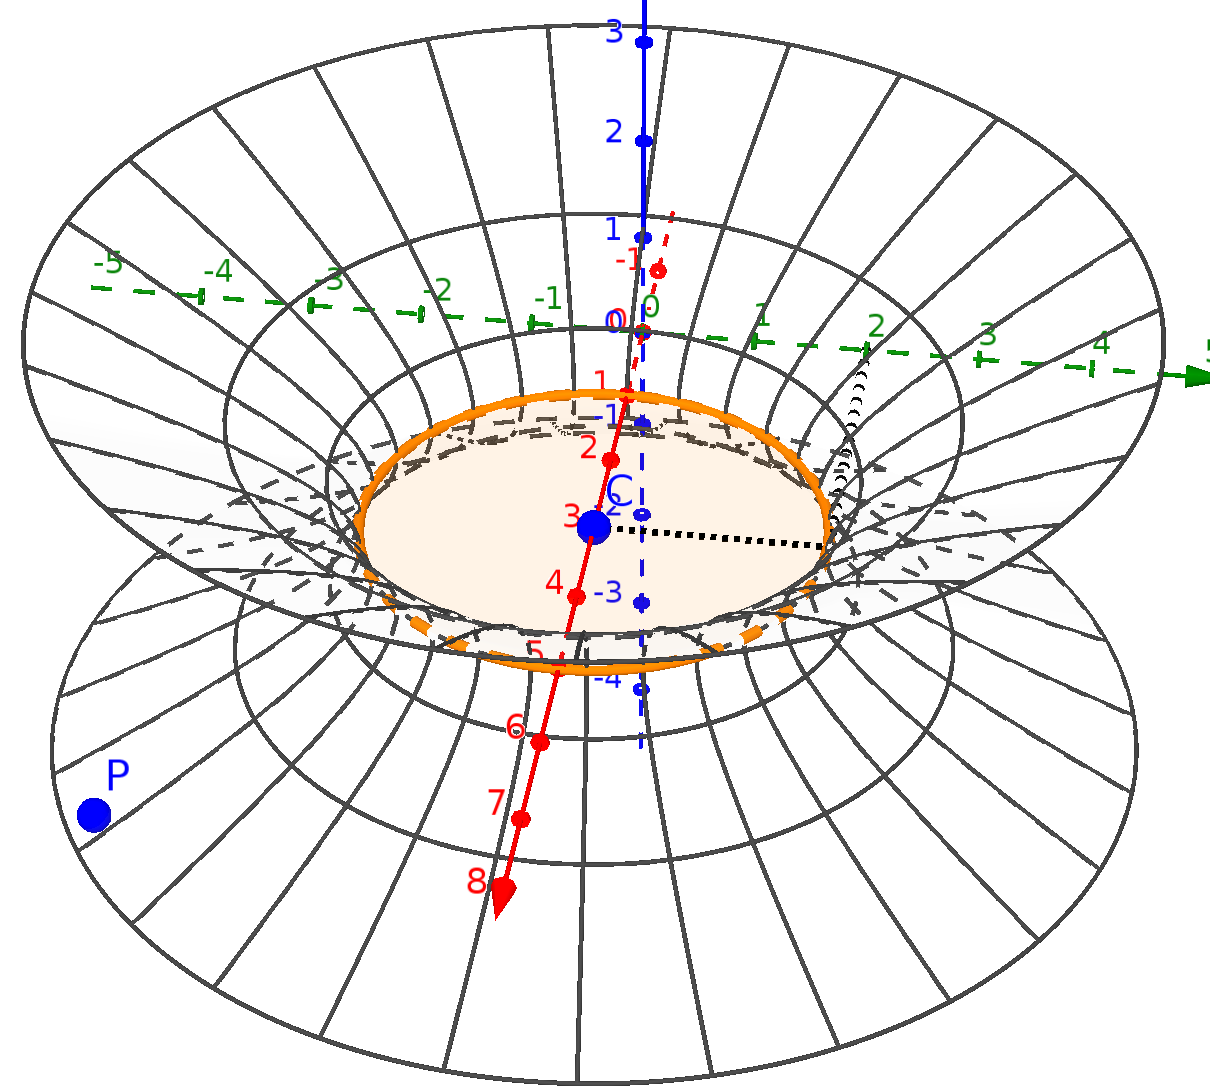
\includegraphics[height=0.90\textwidth]{img/prova-4-pro-hiperboloide-1-folha.png}
        \caption{Superfície}\label{fig:hip-1}
    \end{minipage}
\end{figure}



\Answer \fixme

\Exercise[title={2,5}]
Considere a superfície $S$ dada pela equação $-4x^2 - 4y^2 + z^2 + 8y = 0$.
\begin{enumerate}
\item Que curva é obtida ao intersectar $S$ com o plano $x=0$? E com os planos $z=\pm4$?
\item Identifique o tipo de superfície e represente-a graficamente.
\end{enumerate}
\Answer \fixme

\Exercise[title={2,5}] Considere a superfície quádrica dada pela equação $\dfrac{x^2}{4}-\dfrac{y^2}{36} = 2z$.
\begin{enumerate}
\item Verifique se o ponto $P$ cujas coordenadas cilíndricas são $(3\sqrt{2}, \pi/4, 1)$ pertence à superfície.
\item Verifique se a reta $r:\begin{cases}y=3x+12\\z=-x-2\end{cases}$ está contida na superfície, isto é, se todo ponto de $r$ também pertence à superfície.
\end{enumerate}
\Answer \fixme
\end{ExerciseList}

\begin{center}
BOA PROVA!
\end{center}

%\newpage
\restoregeometry
%\section*{Respostas}
%\shipoutAnswer
\end{document}
